%%%%%%%%%%%%%%%%%%%%%%%%%%%%%%%%%%%%%%%%%%%%%%%%%%%%%%%%%%%%%%%%%%%%%%%%
\section{Introduction}
There has been many measurements (!!!FIXME!!!) about the charge form factor of many elements,
but rarely any precise measurement of the weak form factor of any elements.
The Pb Radius EXperiment-II (PREX-II) and Ca48 Radius EXperiment (CREX) are 
high-precision experiments that measures the tiny asymmetry of polarized electrons
scattered from neutron-rich targets to extract the weak form factor and neutron
skin thickness of those nuclei. In neutron-rich nuclei, the extra nutrons are
pushed out to against the surface tension\cite{PRL.85.5296}, therefore the neutron skin.

With the high-polarization electron beam at 
Thomas Jefferson National Accelerator Facility (TJNAF, also known as Jlab), 
we were able to measure the asymmetry precisely. 
The cross section asymmetry comes from the interference between 
the electromagnetic (EM) interaction and the weak interaction. While the EM 
cross section has been studied thoroughly, (!!!FIXME!!!: reference) the asymmetry 
measurement allows us to derive the weak charge distribution and finally the
neutron distribution in a nuclear.

The measurement of neutron radius of neutron-rich elements is of great importance.
(!!!FIXME: reference)
By constraining the density dependence of the symmetry energy of nuclear matter,
it helps to identify the Equation of State (EoS) of neutron stars.

%%%%%%%%%%%%%%%%%%%%%%%%%%%%%%%%%%%%%%%%%%%%%%%%
\subsection{Asymmetry}
\feynmandiagram[small, vertical' = a to b]{
    i1 [particle = $e^-$] -- [fermion] a -- [fermion] o1 [particle = $e^-$],
    a -- [photon, edge label={Q}, edge label'=$\gamma$] b,
    i2 [particle = p] -- [fermion] b -- [fermion] o2 [particle = p],
    };
\feynmandiagram[small, vertical' = a to b]{
    i1 [particle = $e^-$] -- [fermion] a -- [fermion] o1 [particle = $e^-$],
    a -- [scalar, edge label={Q}, edge label'=Z] b,
    i2 [particle = p] -- [fermion] b -- [fermion] o2 [particle = p],
    };

\begin{itemize}
    \item $\gamma$ interacts with only vector current
    \item while $Z_0$ interacts with both vector and axial-vector current
\end{itemize}

\begin{equation*}
    \CA_{pv} = \frac{\frac{d\sigma^R}{d\Omega} - \frac{d\sigma^L}{d\Omega}}{\frac{d\sigma^R}{d\Omega} + \frac{d\sigma^L}{d\Omega}} = \frac{|\CM^R|^2 - |\CM^L|^2}{|\CM^R|^2 + |\CM^L|^2}
\end{equation*}
where: $\CM^{R, L} = \CM_{\gamma} + \CM_Z^{R,L}$

\begin{equation*}
    \begin{aligned}
	|\CM^{R,L}|^2 &= |\CM_\gamma|^2 + \CM_\gamma\CM_Z^{R,L*} + \CM_\gamma^*\CM_Z^{R,L} + |\CM^{R,L}|^2	\\
	|\CM^{R}|^2 - |\CM^{L}|^2 &= \CM_\gamma( \CM_Z^{R*} - \CM_Z^{L*} + \CM_Z^{R} - \CM_Z^L) \\
	&\approx 2\CM_\gamma(\CM_Z^R - \CM_Z^L)
    \end{aligned}
\end{equation*}


\begin{equation*}
    \begin{aligned}
	\CA_{pv}\footnotemark &\approx \frac{\CM_Z^R - \CM_Z^L}{\CM_\gamma} \propto \frac{\frac{d\sigma_{\text{weak}}}{d\Omega}}{\frac{d\sigma_{\text{E+M}}}{d\Omega}}	\\
	    &\approx \frac{G_F Q^2}{4\pi\alpha\sqrt{2}} \frac{Q_{wk}}{Z}\frac{F_{wk}(Q^2)}{F_{ch}(Q^2)}
    \end{aligned}
\end{equation*}
\begin{equation*}
    \begin{aligned}
	F_{ch}(q) &= G_{ch}^p(q)F_p(q) + G_{ch}^n(q)F_n(q)  \\
		  &= G_E^p(q)F_p(q) + \frac{N}{Z}G_E^n(q)F_n(q)	\\
	F_{wk}(q) &= G_{wk}^p(q)F_p(q) + G_{wk}^n(q)F_n(q)  \\
		  &= G_E^p(q)\left[ F_n(q) - \frac{Z}{N}(1-4\sin^2\theta_W)F_p(q)\right] - G_E^n(q)\left[ F_n(q)(1-4\sin^2\theta_W) - \frac{Z}{N}F_p(q)\right]
    \end{aligned}
\end{equation*}
Where $G_E^p(q)$ and $G_E^n(q)$ are the EW single nucleon FFs, $\sin^2\theta_W = 0.23$ is the Weinberg angle, $F_p(q)$ and $F_n(q)$ are the FFs of point proton and neutron density dist. Compared with $G_E^p(q)$, the charge FF of the neutron $G_E^n(q)$ can be neglected for small momentum transfer:
\begin{equation*}
    \begin{aligned}
	F_p(q) &= \int d^3r j_0(qr) \rho_p(r)	\\
	F_n(q) &= \int d^3r j_0(qr) \rho_n(r)	\\
	G_{wk}^p &= q_p G_E^p + q_n G_E^n + q_0 G_E^s	\\
	G_{wk}^n &= q_p G_E^p + q_n G_E^n + q_0 G_E^s	\\
    \end{aligned}
\end{equation*}
For weak charges including radiative cor.
$$ q_p \approx 0.0712	\qquad q_n = q_0 \approx -0.9877 $$
$$ \frac{F_{wk}(q)}{F_{ch}(q)} \approx \frac{F_n(q)}{F_p(q)}$$
$$ \CA_{pv} = \frac{G_FQ^2}{4\pi\alpha\sqrt{2}}\frac{Q_{wk}}{Z}\left[ \frac{F_n(q)}{F_p(q)} - \frac{Z}{N}(1-4\sin^2\theta_W) \right]$$
where: $F(Q^2) = \int d^3r \frac{sin(Qr)}{Qr}\rho(r)$
\begin{equation*}
    \rho(\vec{r}) = Q^{N}\rho_N(\vec{r}) + Q^{P}\rho_P(\vec{r})
\end{equation*}
In general use model for $\rho(\vec{r})$, example: Wood-Saxon form:
\begin{equation*}
    \rho(r) = \frac{\rho_0}{1 + exp[(r-R)/a]}
\end{equation*}
where R is the radius of the density $\rho(r)$?

\bigskip
When ignoring structure (tree level):
\begin{equation*}
    \CA_{\text{pv}} = \frac{G_F Q^2}{\pi\alpha\sqrt{2}} \left(\sin^2\theta_W + \frac{1}{4}\left[ \frac{N}{Z} - 1 \right] \right)
\end{equation*}
\footnotetext[1]{
    for low $Q^2$:
    \begin{equation*}
	\CA_{pv} = \frac{G_F Q^2}{4\pi\alpha\sqrt{2}} \left[ 1- 4\sin^2\theta_W - \frac{F_n(Q^2)}{F_p(Q^2)} \right]
    \end{equation*}
}

\begin{equation*}
    Q_{\text{weak}}^{p} \propto 1 - 4\sin^2\theta_{\text{W}} \approx 0.076
    \quad
    Q_{\text{weak}}^{n} \propto -1
\end{equation*}
\begin{equation*}
    \sigma_{\text{raw}} = \sigma_{\text{sig}} + \sigma_{\text{other}} + \sigma_{\text{HC}}
\end{equation*}

\begin{equation*}
    \begin{aligned}
	\CA_{\text{pv, measured}} &= \frac{(\sigma_{\text{sig}}^R + \sigma_{\text{other}}^R + \sigma_{\text{HC}}^R) - (\sigma_{\text{sig}}^L + \sigma_{\text{other}}^L - \sigma_{\text{HC}}^L)}{(\sigma_{\text{sig}}^R + \sigma_{\text{other}}^R + \sigma_{\text{HC}}^R) + (\sigma_{\text{sig}}^L + \sigma_{\text{other}}^L - \sigma_{\text{HC}}^L)}    \\
	&\approx \CA_{\text{pv, true}}\left( 1 - \frac{\sigma_{\text{other}}^R + \sigma_{\text{other}}^L}{\sigma_{\text{sig}}^R + \sigma_{\text{sig}}^L} \right) + \frac{\sigma_{\text{HC}}^R + \sigma_{\text{HC}}^L}{\sigma_{\text{sig}}^R + \sigma_{\text{sig}}^L} 
    \end{aligned}
\end{equation*}

\subsection{Dynamics}
\begin{center}
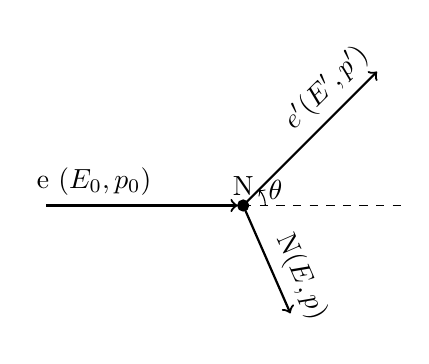
\begin{tikzpicture}
    \coordinate (N) at (0, 0);
    \coordinate (ein) at (-2.5, 0);
    \coordinate (eout) at (1.7, 1.7);
    \coordinate (p) at (0.6, -1.37);

    \filldraw[black] (N) circle (2pt);
    \node [above] at (N) {N};
    \draw[->, thick] (ein) -- node [near start, above] {e ($E_0, p_0$)} ([xshift=-2pt]N);
    \draw[dashed] (N.east) -- +(2, 0);
    \draw[->, thick] (N) -- node[near end, above, sloped] {$e' (E', p')$} (eout);
    \draw[->, thick] (N) -- node[near end, above, sloped] {N($E, p$)} (p);
    \draw [->] ([xshift=8pt]N) arc (0:45:8pt) node[right] {$\theta$};
\end{tikzpicture}
\end{center}

4-Momentum conservation 
$$ E_0 + M = E' + E \qquad \vec{p}_0 = \vec{p}' + \vec{p} $$
Assume ($m_e << 0 \Rightarrow E_0 \approx p_0, E' \approx p'$)
\begin{equation*}
    \begin{aligned}
	E^2 &= M^2 + \vec{p}^2 = M^2 + (\vec{p}_0 - \vec{p}')^2  \\
	    &= M^2 + (E_0 - E'\cos\theta)^2 + (E'\sin\theta)^2	\\
	    &= M^2 + E_0^2 + E'^2 - 2E_0E'\cos\theta	\\
	    &= (E_0 + M - E')^2
    \end{aligned}
\end{equation*}
So we can get
$$ M(E_0 - E') = E_0E'(1-\cos\theta) $$
$$ E' = \frac{ME_0}{M + E_0(1-\cos\theta)}$$
\begin{equation*}
    \begin{aligned}
	Q^2 &= (E_0 - E')^2 - (\vec{p}_0 - \vec{p}')^2	\\
	    &= -2E_0E'(1-\cos\theta)
    \end{aligned}
\end{equation*}

%%%%%%%%%%%%%%%%%%%%%%%%
\subsubsection{Why \Pb and \Ca}
\begin{figure}
    \includegraphics[width=0.5\linewidth]{Nuclear_Landscape}
\end{figure}

%%%%%%%%%%%%%%%%%%%%%%%%%%%%%%%%%%%%%%%%%%%%%%%%
\subsection{Physical Implication}
